%---------------------------------------------------------------------------%
%-                                                                         -%
%-                           LaTeX Template                                -%
%-                                                                         -%
%---------------------------------------------------------------------------%
%- Copyright (C) Huangrui Mo <huangrui.mo@gmail.com> 
%- This is free software: you can redistribute it and/or modify it
%- under the terms of the GNU General Public License as published by
%- the Free Software Foundation, either version 3 of the License, or
%- (at your option) any later version.
%---------------------------------------------------------------------------%
%->> Document class declaration
%---------------------------------------------------------------------------%
\documentclass[twoside]{Style/ucasthesis}%
%- Multiple optional arguments:
%- [<oneside|twoside|print>]% oneside eprint, twoside eprint, or paper print
%- [fontset=<adobe|none|...>]% specify font set instead of automatic detection
%- [scheme=plain]% thesis writing of international students
%- [draftversion]% show draft version information
%- [standard options for ctex book class: draft|paper size|font size|...]%
%---------------------------------------------------------------------------%
%->> Document settings
%---------------------------------------------------------------------------%
\usepackage{caption}
\usepackage[super,numbers, list,table,math]{Style/artratex}
%- usage: \usepackage[option1,option2,...,optionN]{artratex}
%- Multiple optional arguments:
%- [bibtex|biber]% set bibliography processor and package
%- [<numbers|super|authoryear|alpha>]% set citation and reference style
%- <numbers>: textual: Jones [1]; parenthetical: [1]
%- <super>: textual: Jones superscript [1]; parenthetical: superscript [1]
%- <authoryear>: textual: Jones (1995); parenthetical: (Jones, 1995)
%- <alpha>: textual: not available; parenthetical: [Jon95]
%- [geometry]% reconfigure page layout via geometry package
%- [lscape]% provide landscape layout environment
%- [xhf]% disable header and footer via fancyhdr package
%- [color]% provide color support via xcolor package
%- [background]% enable page background
%- [tikz]% provide complex diagrams via tikz package
%- [table]% provide complex tables via ctable package
%- [list]% provide enhanced list environments for algorithm and coding
%- [math]% enable some extra math packages
%- [xlink]% disable link colors
\usepackage{Style/artracom}% user defined commands
%---------------------------------------------------------------------------%
%->> Document inclusion
%---------------------------------------------------------------------------%
%\includeonly{Tex/Chap_1,...,Tex/Chap_N}% selected files compilation
%---------------------------------------------------------------------------%
%->> Document content
%---------------------------------------------------------------------------%
%-
%-> Titlepage information
%-

%---------------------------------------------------------------------------%
%->> Titlepage information
%---------------------------------------------------------------------------%
%-
%-> 中文封面信息
%-
\confidential{}% 密级:涉密论文或延迟公开论文填写
\schoollogo[scale=0.095]{ucas_logo}% 校徽
\title{叶层化代数簇对的Sarkisov纲领}% 论文中文题目
\author{ 王延泽}% 论文作者
\advisor{陈亦飞~副研究员~中国科学院数学与系统研究所\\}% 指导教师:姓名 专业技术职务 工作单位
%\advisor{指导教师一\\指导教师二\\指导教师三}% 多行指导教师示例
\degree{硕士}% 学位:学士、硕士、博士
\degreetype{理学}% 学位类别:理学、工学、工程、医学等
\major{基础数学}% 一级/二级学科专业名称,领域名称需要与学籍信息一致
\institute{中国科学院数学与系统科学研究院}% 院系名称
%\institute{中国科学院力学研究所\\流固耦合实验室}% 多行院系名称示例
\date{2024~年~6~月}% 毕业日期:夏季为6月、冬季为12月
%-
%-> 英文封面信息
%-
\TITLE{Sarkisov program for foliated pairs}% 论文英文题目
\AUTHOR{Yanze Wang}% 论文作者
\ADVISOR{Supervisor: Professor Yifei Chen}% 指导教师
\DEGREE{Master}% 学位:Bachelor, Master, Doctor, Postdoctor。封面据英文学位名称自动切换,需确保拼写准确
\DEGREETYPE{Natural Science }% 学位类别:Philosophy, Natural Science, Engineering, Economics, Agriculture 等
\MAJOR{Pure Mathematics}% 二级学科专业名称
\INSTITUTE{Academy of Mathematics and Systems Science, Chinese Academy of Sciences}% 院系名称
\DATE{June, 2024}% 毕业日期:夏季为June、冬季为December
%---------------------------------------------------------------------------%
%
\begin{document}
%-
%-> Frontmatter: title page, abstract, content list, symbol list, preface
%-

\frontmatter% initialize the environment


%---------------------------------------------------------------------------%
%->> Frontmatter
%---------------------------------------------------------------------------%
%-
%-> 生成封面
%-

\maketitle% 生成中文封面
\MAKETITLE% 生成英文封面
%-
%-> 作者声明
%-
\makedeclaration% 生成声明页
%-
%-> 中文摘要
%-


\intobmk\chapter*{摘\quad 要}% 显示在书签但不显示在目录
\setcounter{page}{1}% 开始页码
\pagenumbering{Roman}% 页码符号

双有理代数几何的目标之一是分类双有理等价类,极小模型纲领用来在每一个固定的双有理等价类中找到一个良好的代表元。
所有这些代表元可以分为两类,一种称为极小模型,另一种称为森纤维空间,两种情况都不唯一。
任何两个MMP-相关的森纤维空间都被一个双有理映射连接,通过运行Sarkisov纲领,可以分解为有限多个基本的双有理映射,这样基本的映射有四种,称为Sarkisov连接。

本文的第一个目标是介绍三种Sarkisov纲领的方法。第二个目标是尝试对叶层化代数簇对建立Sarkisov纲领。通过将$F$-dlt奇点的叶层化代数簇对约化成klt奇点的代数簇对,叶层化森纤维空间之间的双有理映射有较弱的分解。 

\keywords{极小模型纲领,Sarkisov纲领,叶层化代数簇对}% 中文关键词
%-
%-> 英文摘要
%-

\intobmk\chapter*{Abstract}% 显示在书签但不显示在目录

One of goals of birational geometry is to classify birational equivalence classes. The minimal model program  is to find a good representative in every fixed birational equivalence class. 
All of these good representatives can be divided into two classes. One is called the minimal model, and the other is called Mori fiber space, both of  which are not unique. 
Any two MMP-related Mori fibre spaces are connected by a birational map, which can be decomposed into finitely many maps from the four types of elementary birational maps called Sarkisov links, by running the Sarkisov program. 

The first purpose of this paper is to introduce three methods of the Sarkisov program.
The second goal is trying to establish the Sarkisov program for foliated pairs. By reducing $F$-dlt foliated pairs to klt pairs, there is a weak decomposition of birational maps between foliated Mori fibre spaces.  

\KEYWORDS{Minimal Model Program, Sarkisov Program, Foliated pairs}% 英文关键词

% \pagestyle{enfrontmatterstyle}%
\cleardoublepage\pagestyle{frontmatterstyle}%

%---------------------------------------------------------------------------%
% title page, abstract

{% content list region
\linespread{1.2}% local line space
\intobmk*{\cleardoublepage}{\contentsname}% add link to bookmark
\newpage

\tableofcontents% content catalog
\intobmk*{\cleardoublepage}{图表目录}
\pagestyle{figureheader}
{
\cleardoublepage
{
\let\clearpage\relax  % Do nothing when a \clearpage command appears 
\let\cleardoublepage\relax

\renewcommand*{\addvspace}[1]{}
\let\oldnumberline\numberline%
\renewcommand{\numberline}{\figurename~\oldnumberline}%

\listoffigures
\let\clearpage\relax  % Do nothing when a \clearpage command appears 
\let\cleardoublepage\relax
\renewcommand{\numberline}{\appfigname~\oldnumberline}%
\vspace{-30pt}
\listofappfigs
}
{

\let\clearpage\relax  % Do nothing when a \clearpage command appears 
\let\cleardoublepage\relax
\renewcommand*{\addvspace}[1]{}
\let\oldnumberline\numberline%
\renewcommand{\numberline}{\tablename~\oldnumberline}%
\listoftables

\renewcommand{\numberline}{\apptabname~\oldnumberline}%
\vspace{-30pt}
\listofapptabs
}


}


}
\thispagestyle{figureheader}
\intobmk\chapter*{符号列表}% 显示在书签但不显示在目录

\section*{字符}
\nomenclatureitem[\textbf{Unit}]{\textbf{Symbol}}{\textbf{Description}}
\nomenclatureitem[$\Unit{m^{2} \cdot s^{-2} \cdot K^{-1}}$]{$R$}{the gas constant}
\nomenclatureitem[$\Unit{m^{2} \cdot s^{-2} \cdot K^{-1}}$]{$C_v$}{specific heat capacity at constant volume}
\nomenclatureitem[$\Unit{m^{2} \cdot s^{-2} \cdot K^{-1}}$]{$C_p$}{specific heat capacity at constant pressure}
\nomenclatureitem[$\Unit{m^{2} \cdot s^{-2}}$]{$E$}{specific total energy}
\nomenclatureitem[$\Unit{m^{2} \cdot s^{-2}}$]{$e$}{specific internal energy}
\nomenclatureitem[$\Unit{m^{2} \cdot s^{-2}}$]{$h_T$}{specific total enthalpy}
\nomenclatureitem[$\Unit{m^{2} \cdot s^{-2}}$]{$h$}{specific enthalpy}
\nomenclatureitem[$\Unit{kg \cdot m \cdot s^{-3} \cdot K^{-1}}$]{$k$}{thermal conductivity}
\nomenclatureitem[$\Unit{kg \cdot m^{-1} \cdot s^{-2}}$]{$S_{ij}$}{deviatoric stress tensor}
\nomenclatureitem[$\Unit{kg \cdot m^{-1} \cdot s^{-2}}$]{$\tau_{ij}$}{viscous stress tensor}
\nomenclatureitem[$\Unit{1}$]{$\delta_{ij}$}{Kronecker tensor}
\nomenclatureitem[$\Unit{1}$]{$I_{ij}$}{identity tensor}

\section*{算子}
\nomenclatureitem{\textbf{Symbol}}{\textbf{Description}}
\nomenclatureitem{$\Delta$}{difference}
\nomenclatureitem{$\nabla$}{gradient operator}
\nomenclatureitem{$\delta^{\pm}$}{upwind-biased interpolation scheme}

\section*{缩写}
\nomenclatureitem{CFD}{Computational Fluid Dynamics}
\nomenclatureitem{CFL}{Courant-Friedrichs-Lewy}
\nomenclatureitem{EOS}{Equation of State}
\nomenclatureitem{JWL}{Jones-Wilkins-Lee}
\nomenclatureitem{WENO}{Weighted Essentially Non-oscillatory}
\nomenclatureitem{ZND}{Zel'dovich-von Neumann-Doering}

% symbol list, preface content
%-
%-> Mainmatter
%-
\mainmatter% initialize the environment

\chapter{绪论}
\section{主要结果}
双有理代数几何的目标之一是按双有理等价类分类代数簇,并选取选择恰当的代表元。极小模型纲领 (Minimal model program)是构造代表元的一种方法,并且猜想每一个代数簇都双有理等价于一个极小模型 (minimal model) 或一个森纤维空间 (Mori fibre space),但这样的代表元有时并不唯一,于是自然的问题就是不同代表元之间的关系。对于极小模型的情形,我们有
\begin{theorem}[平转连接极小模型]
  令$(W,B_{W})$为一个终端奇点的$\mathbb{Q}$-分解代数簇对,且 $(X,B_{X}), (Y,B_{Y})$是它的两个极小模型。那么双有理映射$X \dashrightarrow Y$可以分解为一系列$(K_{X}+B_{X})$-平转 (flop)的复合。
\end{theorem}

本文主要关注森纤维空间之间的关系:
\begin{theorem}[Sarkisov分解]\label{main}
  令 $ f:(X, B)\to S$ 和 $f':(X', B')\to S' $ 为两个 MMP-连接的klt奇点的$ \mathbb{Q} $-分解森纤维空间,则有双有理映射 $\Phi$:
  \[ \xymatrix{
      (X,B)\ar[d]_{f}\ar@{.>}[r]^\Phi & (X',B')\ar[d]^{f'}\\
      S & S'} \]
  可以分解为Sarkisov连接映射的复合,即
  \[ \Phi=\Psi_{n}\circ \cdots \circ \Psi_{1} \]
  其中$\Psi_{i}:X_{i}\dashrightarrow X_{i+1} $ 是下列四种Sarkisov连接之一:

  \textbf{第一型Sarkisov连接:}
  \[\xymatrix{
      Z\ar[d]_{p}\ar@{.>}[r]&X_{1}\ar[d]^{f_1}\\
      X\ar[d]_{f}&S_1\ar[dl]^{t}\\
  S &}\]
  \textbf{第二型Sarkisov连接:}
  \[\xymatrix{
      Z\ar[d]_{p}\ar@{.>}[r]&Z'\ar[d]^{q}&\\
      X\ar[d]_{f}&X_1\ar[d]^{f_1}\\
  S\ar[r]^{\sim}&S_1}\]
  \textbf{第三型Sarkisov连接:}
\[ \xymatrix{
    X\ar@{.>}[r]\ar[d]_{f}& Z\ar[d]^q& \\
    S\ar[rd]_{s}         & X_{1}\ar[d]^{f_{1}}&\\
    &S_{1}
    } \]
  \textbf{第四型Sarkisov连接:}
\[ \xymatrix{
      X \ar[d]_f\ar@{.>}[rr]&&X_{1}\ar[d]^{f_1}\\
      S \ar[dr]_{s}&&S_{1} \ar[dl]^{t}\\
      &T &} \]
  其中所有$ f:(X, B)\to S $ 和 $ f_1:(X_1, B_1)\to S_1 $ 都是森纤维空间,所有$p,q$ 都是除子压缩,所有虚线的映射都是翻转 (flip)、平转 (flop)或反向翻转 (inverse flip)的复合。
\end{theorem}
这样的分解称为Sarkisov分解,构造这样Sarkisov分解的方法称为Sarkisov纲领。

在叶层化代数簇对 (foliated pair)上有较弱的结果:
\begin{theorem}[弱Sarkisov分解]\label{mainf}
  令$(W,\mathcal{F}_{W},B_{W})$是具有$F$-dlt奇点的$\mathbb{Q}$-分解叶层化代数簇对,且$\rho:W\dashrightarrow X$ 和$\rho':W \dashrightarrow X'$是两个不同的$(K_{\mathcal{F}_{W}}+B_{W})$-MMP的输出,且$X \to S$和$X' \to S'$是两个森纤维空间。那么双有理映射$\Phi:X \dashrightarrow X'$存在分解:
  \[ X=X_{0}\dashrightarrow X_{1}\dashrightarrow \cdots \dashrightarrow X' \]
  每一个代数簇$X_{i}$上有边界除子$D_{i}$和压缩态射$f_{i}:X_{i}\to S_{i}$,使得$(X_{i},D_{i})\to S_{i}$是森纤维空间,并且$X_{i} \dashrightarrow X_{i+1}$是Sarkisov连接。
\end{theorem}

\section{问题的历史}
Sarkisov纲领起源于对直纹曲面的分类 \cite{sarkisovBIRATIONALAUTOMORPHISMSCONIC1981,sarkisovCONICBUNDLESTRUCTURES1983},Matsuki和Reid指出了最初的思路,具有终端奇点的三维代数簇 (terminal threefolds)上的Sarkisov纲领的完整证明由Corti\cite{cortiFactoringBirationalMaps}给出。 

对于双有理同构的两个森纤维空间$X\to S$和 $X'\to S'$,选取$X$ 上一个定义双有理映射$\Phi:X \dashrightarrow X'$的线性系 $\mathcal{H}$ (或一个一般的除子 $H \in \mathcal{H}$),那么第一个Sarkisov连接 $\psi_1:X\dashrightarrow X_1$ 由运行一种特殊的极小模型纲领得到,被称为双射线MMP ($2$-ray game),并且取决于 $\mathcal{H}$ ($H$) 的选取。接着用 $\Phi_{1}=\Phi\circ \psi_1^{-1}: X_1 \dashrightarrow X'$替代 $\Phi:X\dashrightarrow X'$并重复这一过程。通过定义Sarkisov次数,并证明在归纳构造中Sarkisov次数下降来说明归纳终结。Bruno和Matsuki \cite{brunoLogSarkisovProgram1995} 将这种方法推广到klt奇点的 $\mathbb{Q}$-分解三维代数簇的情形,并且对于任意维数的$\mathbb{Q}$-分解klt奇点代数簇对,给出了Sarkisov纲领的大纲和所需要的结论。近年来在极小模型纲领中有一些重要进展,例如标量极小模型纲领 (MMP with scaling) 的终结性 \cite{BCHM10},对数典范阈值 (log canonica threshold, lct)的升链条件 (accending chain condition, ACC)\cite{HMX14}, $\delta$-lc Fano代数簇对的有界性 \cite{Bir19,birkarSingularitiesLinearSystems2020},这些进展使得Bruno和Matsuki的大纲部分地可行,剩下的主要问题与对数翻转的终结性和局部对数典范阈值 (local log canonical thresholds)的ACC (或者有限性)有关。本文将这种方法称为下降法。


利用弱典范模型的有限性\cite{BCHM10} (finiteness of weak log canonical models),Hacon \cite{haconMinimalModelProgram2012} 给出了另一种构造Sarkisov纲领的方法,对所有维数都成立。
这种方法也通过双射线MMP来构造Sarkisov连接,但是固定了两个森纤维空间的公共对数解消 $(W,B_W)$ 作为Sarkisov纲领的``屋顶'',使得分解中的每一个森纤维空间都是$W$的某个弱对数典范模型。双标量法的Sarkisov纲领的终结性由弱对数典范模型的有限性推出,这与标量翻转 (flips with scaling)的终结性的证明类似。
刘继豪 \cite{liuSarkisovProgramGeneralized2021} 将这种方法推广到了一般化代数簇对 (generalized pairs)的情况。本文将这种方法称为双标量法。


利用Shokurov的多面体方法 \cite{Sho96,cs11}, Hacon 和 M\textsuperscript{c}Kernan \cite{haconSarkisovProgram2012}给出了一种新方法,不通过双射线MMP构造Sarkisov连接。
令 $W$ 为 $(X,B)\to S$ 和 $(X',B')\to S'$ 的公共对数解消,则在 $W$ 上有两个除子 $D$ 和 $D'$,使得 $S$ 和 $S'$ 是 $W$ 相对于 $D$ 和 $D'$的丰沛模型 (ample model)。进一步,$W$的除子的多面体的边界上有其他除子 $D_{i}$,每个除子对应一个森纤维空间 $X_{i}\to S_{i}$ 和 $W$的丰沛模型$S_{i}$。在多面体边界上有一条路径连接这些除子 $D_{i}$,并且将$\Phi$分解为对应的Sarkisov连接。
Miyamoto \cite{miyamoto2019TheSP} 将这种方法应用到了任意特征代数闭域上的lc对数曲面或 $\mathbb{Q}$-分解对数曲面。 本文将这种方法称为有限模型法。

\section{本文结构}
第一节给出主要的定理,并介绍Sarkisov纲领的发展历史。第二节给出基本概念的定义,MMP相关的定理。

第三、四、五章分别介绍下降法、双标量法和有限模型法的具体内容,每一章都先介绍这种方法需要的定义和引理,接着说明构造每一个Sarkisov连接的方法,最后说明Sarkisov分解的构造。

在第六章,总结比较三种方法,并且每种方法给出一个具体例子。
% 最后介绍一些Sarkisov纲领的简单应用。

第七章介绍了叶层化代数簇对 (foliated pairs),并分析了三种方法在叶层化代数簇对的推广,最后给出弱化版结果。

\chapter{预备知识}
\section{代数簇对与奇点}
定义代数簇对和相关概念:
\begin{definition}
  定义代数簇对和除子的记号:
  \begin{itemize}
    \item 一个代数簇对 $(X,B)$ 包括一个正规拟射影代数簇 $X$ 和一个 $\mathbb{R}$-除子 $B=\sum_{i}b_{i}B_{i}$,其中$B_{i}$是素除子,且$0<\leqslant b_{i} \leqslant 1$ ,并且满足
    \[ K_{X}+B \]
          是$\mathbb{R}$-Cartier 除子。 
    \item 若双有理态射 $f:Y\to X$ 满足 $Y$是光滑代数簇,且$\operatorname{Exc}\,f \cup \bigcup_{i}B_{i \text{red}} $ 是横截相交 (normal crossing)的除子,并且$f$ 在$\operatorname{Reg}(X,B)$上是同构, 那么称 $f$ 为 $(X,B)$的算术解消。  
    \item 正规代数簇$X$ 的余维数1的不可约子簇$ E \subset X $ 称为 $X$ \textbf{上}的除子;如果 $f: Y \to X$ 是双有理射影态射,那么 $Y$ 上的除子 $E$ 称为 $X$ \textbf{之上}的除子。  
  \end{itemize}
\end{definition}

定义除子的差异数:
\begin{definition}
  令 $(X, B)$ 为代数簇对, 且 $f: Y\to X$ 是它的算术解消,则有
  \[ K_{Y}+C=f^*(K_{X}+B) \]
  那么除子 $E$ 的差异数 (discrepancy)$a(E;X,B) $定义为
  \[ a(E;X,B)=-\operatorname{mult}_{E}C \]
  进一步,定义$(X,B) $的差异数:
  \[ \operatorname{discrep}(X, B) := \inf\{a(E; X, B) : E \text{ 是 } X \text{之上的例外除子} \} \]
  和整体差异数
  \[ \operatorname{totdiscrep}(X, B) :=\inf \{a(E; X, B) : E \text{是} X \text{之上的除子}\}. \]
\end{definition}
对于代数簇对之间的态射,可以定义
\begin{definition}
 令$f:(Y,C)\to (X,B)$ 为代数簇对之间的态射,在分歧公式中,
 \[ K_{Y}+C + \sum_{i}e_{i}E_{i}=f^{*}(K_{X}+B) \]
 如果$e_{i}=0$,那么除子$E_{i}$称为$f$-相容的。 如果
 \[ K_{Y}+C=f^{*}(K_{X}+B) \]
那么称$f$ 是\textbf{无差别的},也称为\textbf{相容的}  (crepant)。
如果考虑不含边界的代数簇对,即$B=C=0$ ,那么分歧公式
 \[ K_{Y} + \sum_{i}e_{i}E_{i}=f^{*}K_{X} \]
 中满足$e_{i}=0$的除子称为无差别除子。
\end{definition}

通过差异数,定义代数簇对 $(X,B)$ 的奇点性质:
\begin{definition}
  对于代数簇对$(X,B)$,定义奇点性质:
  \begin{itemize}
    \item 如果 $\operatorname{discrep}(X,B)>0$,则称$(X,B) $具有终端奇点 (terminal),也称 $K_{X}+B$具有终端奇点; 
    \item 如果 $\operatorname{discrep}(X,B)\geqslant 0$,则称$(X,B) $具有典范奇点 (canonical),也称 $K_{X}+B$具有典范奇点; 
    \item 如果 $\operatorname{discrep}(X,B)>-1$,则称$(X,B) $具有klt奇点 (kawamata log terminal),也称 $K_{X}+B$具有klt 奇点; 
    \item 如果 $\operatorname{discrep}(X,B)\geqslant -1$,则称$(X,B) $具有lc奇点 (log canonical),也称 $K_{X}+B$具有lc奇点; 
    \item 如果 $\operatorname{discrep}(X,B)\geqslant -1+\delta$,则称$(X,B) $具有$\delta$-lc奇点,也称 $K_{X}+B$具有$\delta$-lc奇点; 
  \end{itemize}
\end{definition}

\section{极小模型纲领}

\begin{theorem}[锥定理]\label{conethm}

令$(X,B)$ 是具有klt奇点的$\mathbb{Q}$-分解代数簇对,且$(K_{X}+B)$不是数值有效的,那么有
\begin{enumerate}
  \item
    \[ \overline{\operatorname{NE}}(X)=\overline{\operatorname{NE}}(X)_{K_{X}+B\geqslant 0} +\sum_{\alpha \in\Lambda} R_{\alpha}\] 
          其中$R_{\alpha}=\mathbb{R}_{\geqslant 0}[C_{\alpha}]$是由有理曲线$C_{\alpha}$生成的$(K_{X}+B) $-负性的极端射线,且$\Lambda$是可列集;
  \item 对任何丰沛除子$A$和$ \epsilon >0 $,有
        \[ \overline{\operatorname{NE}}(X)=\overline{\operatorname{NE}}(X)_{K_{X}+B+\epsilon A\geqslant 0} +\sum_{\alpha \in\Lambda'}R_{\alpha} \]
        其中$\Lambda' \subset \Lambda$是有限子集;
  \item 令 $F \subset \overline{\operatorname{NE}}(X)$是 $(K_{X}+B)$-负性的极端面,那么同构意义下存在唯一的压缩态射
    \[ f=cont_{F}:X \to Z \]
    使得$f_{*}\mathcal{O}_{X}=\mathcal{O}_{Z}$,并且曲线 $C \subset X$被$f$ 压缩当且仅当$[C] \in F$。 
  \item 如果$X$ 上除子 $D$,相对于$Z$ 是数值平凡的,即任意被$f$ 压缩的曲线$C \subset X$,都有$D.C=0$,那么存在$Z$上除子$L_{Z} $使得
    \[ f^{*}L_{Z} = D \]
\end{enumerate}
\end{theorem}
当$F=R$是极端射线时,有$\rho(X)=\rho(Z)+1$。压缩态射$f$有三种情况:
\begin{enumerate}
  \item $\operatorname{Exc}\,f=E$是素除子,此时称为除子压缩;
  \item $\operatorname{codim }(\operatorname{Exc}\,f) \geqslant 2$,则称为小双有理态射 (small birational morphism);
  \item $\dim Z < \dim X, \operatorname{Exc}\,f=X$,此时称$(X,B)\to Z$为森纤维空间 (关于$ (K_{X}+B) $的森纤维空间),压缩态射$f$称为森纤维空间压缩态射。
\end{enumerate}
\textbf{极小模型纲领 (MMP):}
对于$(X,B)=(X_{0},B_{0})$,应用锥定理做关于极端射线的压缩态射$f_{1}:X\to Z$。
\begin{enumerate}
  \item 如果是除子压缩,那么令$X_{1}=Z,B_{1}=f_{1*}B$。在$(X_{1},B_{1})$上重复此过程;
  \item 如果是小双有理态射,那么令$f^{+}_{1}:X_{1}\to Z$为$f_{1}$的翻转 (flip),并记$B_{1}$为$B$ 在$X_{1}$上的严格双有理变换。在$(X_{1},B_{1})$上重复此过程;
  \item 如果是森纤维空间压缩,那么MMP停止。
\end{enumerate}
如果持续做前两种操作,并最终在$(X_{i},B_{i})$上$K_{X_{i}}+B_{i}$是数值有效除子,那么MMP在此终结,且$(X_{i},B_{i})$是极小模型;
如果在森纤维空间$(X_{i},B_{i})\to Z$停止,那么MMP终结于这个森纤维空间。


MMP中出现的代数簇对被称为极小模型的\textbf{结果},将MMP停止处的代数簇称为MMP的\textbf{输出} (要么是极小模型,要么是森纤维空间)。对于极小模型纲领,有如下结果。
\begin{theorem}[标量MMP的终结定理]
  \cite[Corollary 1.4.2]{BCHM10} 令 $ \pi: X\to U $ 为正规拟射影代数簇间的射影态射,且 $(X, B)$ 是  $\mathbb{Q}$-分解的具有 klt奇点的 代数簇对,其中 $K_{X}+B$  $\mathbb{R}$-Cartier 除子, 且$B$ 是 $\pi$-big。若 $C\geqslant0$ 为 $\mathbb{R}$-除子,且$K_{X}+B+C$ 具有 klt奇点 且  $\pi$-数值有效 (nef),那么在 $U$ 上运行 $C$-标量的  $(K_{X}+B)$-MMP,那么这个极小模型纲领将终结。
\end{theorem}

如果$(K_{X}+B)$-MMP终结,那么其输出和$(K_{X}+B)$有下列关系:
\begin{theorem}[极小模型输出]\label{notpseudoeffmfs}
  \cite[Corollary 1.3.3]{BCHM10} 令 $ \pi: X\to U $ 为正规拟射影代数簇间的射影态射,且 $(X, B)$ 是 $\mathbb{Q}$-分解 klt 代数簇对,其中 $K_{X}+B$ 是$\mathbb{R}$-Cartier 除子。若 $K_{X}+B$ 不是 $\pi$-伪有效的,那么运行 $U$ 上的  $(K_{X}+B)$-MMP,将终结于森纤维空间$g:Y\to Z$。
\end{theorem}
注意到如果$ \pi:X \to Y$是双有理射影态射,那么$X$ 上所有除子都是相对于$Y$ 的大除子,于是有以下推论:   
\begin{corollary}\label{extraction}
  \cite[Corollary 13.7]{haconMinimalModelProgram2012} 令 $ (X,B) $ 为 klt 代数簇对, $\mathfrak{C}$是任意差异数满足 $ a(E;X,B)\leqslant 0 $的例外除子 $E$ 的集合,那么有双有理态射 $ f:Z\to X $ 和 $ \mathbb{Q} $-除子 $ B_Z $ 使得:
  \begin{enumerate}
    \item $ (Z,B_Z) $ 是klt代数簇对:
    \item $ E $ 是 $f$-例外除子当且仅当 $ E\in \mathfrak{C} $;
    \item  若 $E \in \mathfrak{C}$则$ \operatorname{mult}_{E}B_Z=-a(E;X,B) $ ,且$ f_*B_Z=B $ 和 $ K_Z+B_Z=f^*(K_X+B) $。
  \end{enumerate}
  特别的,若设 $\mathfrak{C}$ 为所有差异数满足$a(E; X, B)\leqslant 0$的例外除子 $E$ 的集合,那么 $ Z $ 被称为 $X$ 的 \textbf{终端化} (terminalization) ;若取 $\mathfrak{C}$为仅包含一个差异数满足 $a(E; X, B)\leqslant 0$的例外除子,那么 $ f: Z\to X $ 被称为 \textbf{除子解压} (\textbf{divisorial extraction}).
\end{corollary}
对相同的代数簇对$(X,B)$和算术典范除子$K_{X}+B$,对应的$(K_{X}+B)$-MMP可能有不同的输出,它们之间有下列关系:
\begin{definition}
  \cite[Definition 3.3]{brunoLogSarkisovProgram1995}
  如果多个代数簇对 $ \{(X_i,B_i)\} $是从算术光滑的代数簇对 $(W,B_{W})$的 $(K_{W}+B_{W}) $-MMP的不同结果,则称它们为MMP-相关的 ( \textbf{MMP-related} )。 
\end{definition}

\begin{lemma}\label{MMPrelatedConditation}
  \cite[Proposition 3.4]{brunoLogSarkisovProgram1995}
  令 $ \{(X_l,B_l)\} $ 为有限多个互相双有理等价的 $ \mathbb{Q} $-分解 klt 代数簇对,那么下列条件等价:
  \begin{enumerate}
    \item 它们是MMP-相关的;
    \item 存在一个算术光滑代数簇对 $ (W,B_W) $和一组射影双有理态射  $ f_l:W\to  X_l $ 支配每个 $ X_l $,满足 $ f_{l*}B_W=B_l $ 和分歧等式
      \[ K_W+B_W=f_l^*(K_{X_l}+B_l)+\sum_{\text{例外除子}E_{li}}{a_{li}E_{li}} \]
          其中对每个$ f_l $-例外除子$E_{li}$满足 $a_{li}>0$ 的不等式条件;
    \item 对任意两个代数簇对 $ (X,B=\sum_ib_{i }B_i),(X',B'=\sum_{j}b_{j}'B_{j}') $ , 有  $ a(B_i;X',B')\geqslant -b_i $ 且严格不等式成立当且仅当 $ B_i $ 是 $ X' $上的例外除子。同样的,有 $ a(B'_j;X,B)\geqslant -b'_j $ 且严格不等式成立当且仅当$ B'_j $ 是 $ X $上的例外除子。
  \end{enumerate}
\end{lemma}
\begin{proof}
  我们给出  $(3) \implies (2)$的简略证明:令 $W$ 为支配每个代数簇对 $(X_l,B_l=\sum b_{li}B_{li})$ 的算术光滑解消,并有射影双有理态射 $f_l:W\to X_l$,它们例外除子的并$f_{l*}^{-1}B_l\cup E_{li}$是一个横截相交的除子。令 $B_W=\sum_t d_tD_t $,其中  如果 $D_t$ 是$\cup_l f_{l*}^{-1}B_l$中的某个素除子则$d_t = b_{li}$,如果$B_{t}$是每个 $X_{l}$上的例外除子,则  $d_t=1$。由条件(3), 这是定义良好的。那么 $(W,B_{W})$上的分歧等式(ramification formula)中的不等式条件也由(3)得到。
\end{proof}

\section{模型及其有限性}

\begin{definition}
  \cite[\S 2]{haconSarkisovProgram2012} 对有理映射 $f:X\dashrightarrow Y$  若有 $f$的解消$p:W\to X$ 和 $q:W\to Y$ 满足$p$  和 $q$ 都是压缩态射且 $p$ 双有理态射,则称 $f$ 为有理压缩映射( \textbf{rational contraction})  。若 $ q$也是双有理态射, 且每个 $p$-例外除子都是 $q$-例外除子,则称 $f$为双有理压缩映射 (\textbf{birational contraction})。如果 $f^{-1}$ 也是双有理压缩映射,则称 $f$ 为小双有理映射   ( \textbf{small birational map} )。
\end{definition}

\begin{definition}\label{negativemap}
  \cite[Definition 3.6.1]{BCHM10}令 $f:X\dashrightarrow Y$为正规拟射影代数簇间的双有理映射,且 $p:W\to X$ 和 $q:W\to Y$是 $f$的解消。若 $D$是 $X$ 上的$\mathbb{R}$-Cartier 除子,满足  $D_{Y}=f_*D$ 也是 $\mathbb{R}$-Cartier除子,那么如果满足
  \begin{itemize}
    \item $f$ 不解压任何除子(即 $f$ 是双有理压缩 );
    \item $E=p^{*}D-q^*D_Y$ 是  $Y$上的有效除子 (对应的, $\operatorname{Supp}p_*E$ 包含全部 $f$-例外除子)。
  \end{itemize}
 则称$f$为 $D$-非正性的  (\textbf{$D$-non-positive}) ,对应的, $D$-负性的 ( \textbf{$D$-negative)}。
\end{definition}

回顾双有理代数几何中关于模型的定义 \cite{BCHM10}:
\begin{definition}
  \cite[Definition 3.6.5]{BCHM10} 令 $ \pi:(X,D)\to U $为正规拟射影代数簇间的射影态射, $K_{X}+D$ 是 $X$ 上的$\mathbb{R}$-Cartier除子,且$ f: X\dashrightarrow Y $是 $U$ 上的双有理映射。  如果 $ f $ 是 $ (K_X+D) $-非正性的且 $ K_Y+f_*D $ 是 $ U $上半丰沛的,那么称 $Z$ 和 $f$ 为关于 $D$的\textbf{半丰沛模型}(\textbf{semiample model})。

  令 $ g:X\dashrightarrow Z $ 为$ U $上的有理映射,$p:W \to X $ 和 $q:W \to Z $是对 $g$ 的解消,其中 $q$ 是压缩态射 。 若$Z$ 上有 $U$ 上的丰沛除子 $H$ ,且 $p^*(K_{X}+D) \sim_{\mathbb{R},U} q^*H+E$ ,其中 $E$  满足    对 任意的 $B \in |p^*(K_{X}+D)/U|_{\mathbb{R}}$都有 $B\geqslant E$,则称 $Z$ 是 $X$ 关于$D$ 的\textbf{丰沛模型} (\textbf{ample model}) 。
\end{definition}

\begin{remark}
  在原文献和其他文献中的常见定义如下:令 $ \pi:X\to U $为正规拟射影代数簇间的射影态射, $D$ 是 $X$ 上的$\mathbb{R}$-Cartier除子,且$ f: X\dashrightarrow Y $是 $U$ 上的双有理映射。  如果 $ f $ 是 $ D $-非正性的且 $ f_*D $ 相对于 $ U $是半丰沛的,那么称 $Z$ 和 $f$ 为关于 $D$的\textbf{半丰沛模型}(\textbf{semiample model})。

  但本文中只考虑$D=K_{X}+B$是算术典范除子的情况,并且为记号简便做此修改。丰沛模型、弱算术典范模型等都做此修改。
\end{remark}
\begin{definition}\label{models}
  \cite[Definition 3.6.7]{BCHM10} 令 $ \pi:(X,D)\to U $为正规拟射影代数簇间的射影态射,若 $ K_X+D $ 是 lc且$ f:X\dashrightarrow Y $是双有理压缩映射,那么有如下定义:
  \begin{enumerate}
    \item 如果 $f$ 是  $ (K_X+D) $-非正性的且 $ K_Y+f_*D $ 是 $ U $上数值有效的,则  称$ Y $为关于 $D$ 在 $U$上 的  \textbf{弱算术典范模型}(\textbf{weak log canonical model});
    \item 如果 $f$ 是  $ (K_X+D) $-非正性的且 $ K_Y+f_*D $ 是 $ U $上丰沛的,则  称$ Y $为关于 $D$ 在 $U$ 上的  \textbf{算术典范模型}(\textbf{ log canonical model});
    \item 如果 $f$ 是  $ (K_X+D) $-负性的且 $ K_Y+f_*D $ 是 $ U $上数值有效的和$\mathbb{Q}$-分解的,并且具有dlt奇点,则  称$ Y $为关于 $D$ 在 $U$上的  \textbf{算术终端模型}(\textbf{log terminal model})。
  \end{enumerate}
\end{definition}

\begin{lemma}\cite[lemma 3.6.6]{BCHM10}
  令 $\pi:X \to U$ 是正规拟射影代数簇间的射影态射,且 $D$是 $X$ 上的 $\mathbb{R}$-Cartier除子。

  \begin{enumerate}
    \item 如果 $g_{i}:X \dashrightarrow X_{i}, i=1,2$ 是 关于 $D$的  $U$上的两个丰沛模型,那么有同构态射 $h:X_{1}\to X_{2}$ 满足 $g_{2}=h \circ g_{1}$。即丰沛模型在同构意义下唯一。
    \item 如果 $f:X \dashrightarrow Y$是 $U$ 上关于 $D$ 的 半丰沛模型,那么 $U$ 上关于 $D$ 的丰沛模型 $g:X \dashrightarrow  Z$存在,并且 $g=h \circ f$,其中 $h:Y \to Z$是压缩态射, $Z$ 上有对应丰沛除子 $H$  满足$f_*D \sim_{\mathbb{R},U}h^*H$。
    \item  若 $f:X \dashrightarrow Y$  是$U$上双有理映射,那么 $f$是关于$D$ 在 $U$上的丰沛模型当且仅当$f$是关于 $D$ 在 $U$ 上的  半丰沛模型 且 $f_*D$ 在 $U$上丰沛。
  \end{enumerate}
\end{lemma}
根据上述引理,有算术典范模型的等价定义:

\begin{definition}
  令 $ \pi:(X, D)\to U $是正规拟射影代数簇间的射影态射,$ K_X+D $ 有lc奇点且$ f: X\dashrightarrow Y $ 是不解压任何除子的双有理映射。 如果 $ Y $是 关于 $D$ 在 $U$ 上的丰沛模型,那么称之为\textbf{算术典范模型} ( \textbf{log canonical model} ) 。
\end{definition}

进一步,对于边界是大除子的代数簇对,还有
\begin{lemma}\cite[lemma 3.9.3]{BCHM10} 令 $ \pi:(X,B)\to U $是正规拟射影代数簇间的射影态射,且 $(X, B)$是具有klt 奇点的代数簇对,  $B$ 在 $U$上是大除子。如果 $f:X\dashrightarrow Y$是 $U$ 上 弱算术典范模型,那么
  \begin{itemize}
    \item $f$ 是$U$上半丰沛模型;
    \item  $U$ 上的丰沛模型  $g:X \dashrightarrow Z$存在;
    \item  存在压缩态射$h:Y\to Z$和 $Z$ 上在 $U$ 上丰沛的$\mathbb{R}$-除子,使得 
      \[ K_{Y}+f_*B\sim_{\mathbb{R},U} h^*H \]
  \end{itemize}
\end{lemma}
下面给出除子的多面体相关的定义和定理:
\begin{definition}\label{polytopeofdivisor}
  \cite[Definition 1.1.4]{BCHM10} 令 $ \pi: X\to U $ 为正规拟射影代数簇间的射影态射,且 $ V $是 $ \operatorname{WDiv}_{\mathbb{R}}(X) $的定义在有理数上的优先为子射影空间。取定一个 $ \mathbb{R} $-除子 $ A\geqslant 0 $,定义:
  \[
    \begin{aligned}
      \mathcal{L}_A(V)       & =\{D=A+B:B \in V,  K_X+D\, \text{有lc奇点且} B\geqslant0 \} \\
    \mathcal{E}_{A,\pi}(V) & =\{D\in \mathcal{L}_A(V): K_X+D\, \text{ 是 } U \text{上的伪有效除子}\}  \\
    \end{aligned}
  \]
  令 $ f:X \dashrightarrow Y$为 $U$ 上的 双有理压缩映射,定义
  \[ \mathcal{W}_{A,\pi,f}(V)=\{D\in \mathcal{E}_{A}(V): f \text{是   } (X,D) \text{ 在 }U \text{上的弱算术典范模型}\} \]
  令 $g:X\dashrightarrow Z  $ 是 $ U $上的有理压缩映射,定义
  \[ \mathcal{A}_{A,\pi,g}(V)=\{D\in \mathcal{E}_{A}(V): g \text{是} (X,D) \text{ 在 }U \text{上的丰沛模型}\} \]
  进一步,将 $ \mathcal{A}_{A,\pi,g}(V) $ 在 $\mathcal{L}_{A}(V)$中的闭包记作 $ \mathcal{C}_{A,\pi,g}(V) $。

  如果基底 $U$是清楚的,或是一个点,那么我们省略 $\pi$,简单记作 $\mathcal{E}_{A}(V)$ 和 $\mathcal{A}_{A,f}$。
\end{definition}

\begin{theorem}\label{finitewlcm}
  (弱算术典范模型有限性, \cite[Theorem E]{BCHM10}).
  令 $\pi: X\to U$是正规拟射影代数簇间的射影态射,且$A$是一个一般的 在 $U$ 上丰沛的$\mathbb{R}$-除子,且$V \subset \operatorname{WDiv}_{\mathbb{R}}(X)$是定义在有理数上的有限维线性子空间,假设存在具有klt奇点的代数簇对 $(X,\Delta_{0})$。那么存在有限多个 $U$ 上的 双有理映射 $f_{i}:X \dashrightarrow X_{i},1\leqslant i\leqslant l$ ,若某个 $D \in \mathcal{L}_{A}(V)$ 有关于 $D$ 的在 $U$ 上的  弱算术典范模型 $f:X \dashrightarrow  Y$,那么对某个$1\leqslant i\leqslant l$存在同构态射  $h_{i}:X_{i} \to Y$ 使得 $f=h_{i}\circ f_{i}$。
\end{theorem}

\chapter{Sarkisov纲领}


\section{双标量法}

\section{有限模型法}



\chapter{叶层化Sarkisov纲领}
用子层$\mathcal{F} \subset \mathcal{T}_{X}$ 代替切丛,进而用叶层化典范除子 (foliated canonical divisor) $K_{\mathcal{F}}$代替典范除子$K_{X}$,并且有对应的叶层化极小模型纲领,在高维情况下尤其对代数可积的叶层化代数簇对有一系列结果。本章尝试分析这种情况下的Sarkisov纲领。
\section{定义和引理}
首先给出\textbf{叶层化代数簇对} (或 \textbf{带叶状结构的代数簇对})的基本知识。

\begin{definition}[叶状结构]\cite[Definition 2.3-6]{acc_foliation}
  \begin{enumerate}
    \item 令 $X$ 为正规代数簇。$X$ 上的一个叶状结构 (folation)是一个凝聚层 $\mathcal{F} \subset \mathcal{T}_{X}$,满足
          \begin{enumerate}
            \item $\mathcal{T}_{X}/\mathcal{F}$是无扭的 (torsion free);
            \item $\mathcal{F}$在李括号下封闭。 
          \end{enumerate}
          如果$\mathcal{F}=0$,称之为由点定义的叶状结构 (此时此叶状结构的叶子 (leaves)是单点)。
    \item 对$X$ 上素除子 $D$,若$D$ 不是 $\mathcal{F}$-不变的,则定义$\epsilon_{\mathcal{F}}(D)=1 $;反之,如果$D$ 是$\mathcal{F}$-不变的,则定义$\epsilon_{\mathcal{F}}(D)=0$。
    \item 如果除子$K_{\mathcal{F}}$满足$\det \mathcal{F} = \mathcal{O}_{X}(-K_{\mathcal{F}})$,则称之为$\mathcal{F}$的典范除子。
    \item 令$f:X \dashrightarrow Y$为支配有理映射,将$X$ 上的叶状结构$\mathcal{F}$的在$f$ 的拉回记作  $ f^{-1}(F) $ (叶状结构的拉回的定义,参考\cite[3.1]{acss} 或\cite[3.2]{cs21}),并且称其为$\mathcal{F}$诱导的 $\mathcal{Y}$ 上的叶状结构。令$g:X \dashrightarrow X' $为双有理映射,则将$(g^{-1})^{-1}(\mathcal{F})$记为 $g_{*}\mathcal{F}$,并称为$\mathcal{F}$的推出。
    \item 如果存在支配有理映射$h:X \dashrightarrow  Z$和$Y$ 上的由点定义的叶状结构$\mathcal{F}_{Z}=0$  ,使得  $\mathcal{F}=h^{-1}(\mathcal{F}_{Z})$,则称$\mathcal{F}$为代数可积 (algebraically integrable)的叶状结构,并且称$\mathcal{F}$由$h$ 诱导。 
  \end{enumerate}
\end{definition}
用$K_{\mathcal{F}}$代替$K_{X}$,可以定义相应的概念
\begin{definition}
使用\cite[3.4.5,6.2.1]{chlx}、\cite[3.2]{acss}的定义:
  \begin{enumerate}
    \item 叶层化代数对 $(X/U,\mathcal{F},B)$包括一个正规射影代数簇$X$ ,叶状结构$\mathcal{F}$和边界除子$B$,一个压缩态射$\pi:X\to U$,使得叶层化算术典范除子
  \[ K_{\mathcal{F}}+B \]
  是$\mathbb{R}$-Cartier除子。当基底$U=pt$,或清楚时,常舍去$U$,简记为$(X,\mathcal{F},B)$。 
    \item 如果$f:Y\to X$是双有理态射,且$\mathcal{F}_{Y} $是$\mathcal{F} $诱导的 $Y$ 上的叶状结构,且$E \subset Y$是$Y$ 上的除子,那么分歧公式
  \[ K_{\mathcal{F}_{Y}}+C=f^{*}(K_{\mathcal{F}}+B) \]
  定义了例外除子$E$的叶层化差异数
  \[ a(E;X,\mathcal{F},B)=- \operatorname{mult}_{E}C \]
    \item 用叶层化差异数可以定义奇点性质:
      \begin{enumerate}
        \item 如果对所有除子$E$,有 $a(E;X,\mathcal{F},B)>-\epsilon(E)$,则称$(X,\mathcal{F},B) $具有klt奇点;
        \item 如果对所有除子$E$,有 $a(E;X,\mathcal{F},B)\geqslant -\epsilon(E)$,则称$(X,B) $具有lc奇点 ;
      \end{enumerate}
    \item 代数可积的叶层化代数对$(X,\mathcal{F},B)$如果满足:
      \begin{enumerate}
        \item $X$最多有商奇点 (quotient singularities);
        \item 存在压缩态射$f:X\to Z$,使得$\mathcal{F}$是由$f$ 诱导的叶状结构; 
        \item 存在一个约化除子$\Sigma$使得$\operatorname{Supp}B \subset \operatorname{Supp} \Sigma $,且 $(X,\Sigma)$是环形的 (toroidal),特别的,$X$是$\mathbb{Q}$-分解的具有klt奇点的代数簇;
        \item 存在约化除子$\Sigma_{Z}$使得$ (Z,\Sigma_{Z})$是算术光滑的,并且
          \[ (X,\Sigma)\to (Z,\Sigma_{Z}) \]
          是等维数环形态射 (equidimensional toroidal morphism)
      \end{enumerate}
      则称为叶层化算术光滑代数对。
    \item 对代数可积叶层化代数簇对$(X,\mathcal{F},B)$,如果有双有理态射$f:Y\to X$,使得
      \[ (Y,\mathcal{F}_{Y}=f^{-1}\mathcal{F},B_{Y}=f^{-1}_{*}B+ \operatorname{Exc}f) \]
      是叶层化算术光滑代数簇对,那么称$f$为叶层化算术解消 (foliated log resolution)。
    \item 对具有lc奇点的代数可积叶层化代数簇对$(X,\mathcal{F},B)$,如果有叶层化算术解消$f:Y\to X$,使得任意$X$ 上例外除子$E \subset Y$,都有
      \[ a(E;X,\mathcal{F},B)>-\epsilon_{\mathcal{F}}(E) \]
      那么称其具有$F$-dlt奇点。
  \end{enumerate}
\end{definition}
在叶层化代数簇对中,还有一种特殊的奇点性质,首先由Ambro, Cascini, Shokurov, Spicer在\cite{acss}中提出:
\begin{definition}[ACSS奇点]\cite[Definition 4.1-3]{acc_foliation}
 设$ (X/U,B) $为具有lc奇点的代数簇对,且$f: X\to Z$是压缩态射。记$B^{v}$和$ B^{h}$分别为$B$ 在$Z$ 上垂直和水平的部分,即$B^{v}$ 的组成成分素除子$D$满足$f(D)\subsetneq Z $,而$B^{h}$  的组成成分素除子$D$满足$f(D)= Z$。如果满足下列性质:
 \begin{enumerate}
   \item 存在$Z$ 上的约化除子$\Sigma_{Z}$,使得$(Z,\Sigma_{Z}) $是算术光滑代数簇对,且$f(B^{v}=\Sigma_{Z})$;
   \item 对任意闭点$z \in Z$和约化除子$\Sigma \geqslant \Sigma_{Z}$,如果$(Z,\Sigma)$在$z \in Z$附近是算术光滑的,那么$(X,B+f^{*}(\Sigma-\Sigma_{Z}))$在$z \in Z$附近具有lc奇点。 
 \end{enumerate}
 那么称$(X/U,B)/Z$具有性质$*$。

 对于代数可积的叶层化代数簇对$(X/U,\mathcal{F},B)=(X,\mathcal{F},B)$,如果存在压缩态射$f:X \to Z$和约化除子$G$,满足下列条件
 \begin{enumerate}
   \item $(X/U,B+G)/Z$满足性质$*$;
   \item $\mathcal{F}$由$ f$诱导;
   \item $G$是$\mathcal{F}$-不变除子 (在这种情况下,等价于$G$在$Z$上垂直)
 \end{enumerate}
那么称$(X/U,\mathcal{F},B;G)/Z$具有性质$*$。进一步,如果还满足
\begin{enumerate}
  \item $(X/U,\mathcal{F},B)$具有lc奇点;
  \item $f$是等维数压缩态射
\end{enumerate}
则称$(X/U,\mathcal{F},B;G)/Z$满足弱ACSS条件,或者具有弱ACSS奇点。如果还满足
\begin{enumerate}
  \item 如果除子$\Sigma \subset Z$满足$\Sigma \geqslant f(G)$且$(Z,\Sigma)$是算术光滑代数簇对,那么
    \[ (X/U,\mathcal{F},B+G+f^{*}(\Sigma - f(G ))) \]
  \item 如果$W$是lc中心,且$ \eta_{W}$是一般点 (generical point),那么$(X,B+G)$在$\eta_{W}$附近是环形的,且$W$ 是$(X/U,\mathcal{F},\left\lfloor B \right\rfloor )$的lc中心。
\end{enumerate}
那么称具有ACSS性质,或具有ACSS奇点。
\end{definition}
这种奇点在叶层化MMP下保持:
\begin{proposition}\cite[Lemma 4.8]{acc_foliation}\label{acssmmp }
 设$(X/U,\mathcal{F},B;G)/Z$具有ACSS奇点,并且是$\mathbb{Q}$-分解的。那么 
 \begin{enumerate}
   \item 任何$(K_{\mathcal{F}}+B)$-负性的相对于$U$的极端射线都是 $(K_{X}+B+G)$-负性的相对于$Z$ 的极端射线,因此每一步相对于$U$ 的 $(K_{\mathcal{F}}+B)$-MMP都是相对于$Z$ 的$(K_{X}+B+G)$-MMP;
   \item 如果$\phi:(X,\mathcal{F},B;G) \dashrightarrow (X',\mathcal{F}',B';\phi_{*}G)$是一部$(K_{\mathcal{F}}+B)$-MMP,那么$(X',\mathcal{F}',B';\phi_{*}G)$也是$\mathbb{Q}$-分解的具有ACSS奇点的代数可积叶层化代数簇对。
 \end{enumerate}
\end{proposition}
$F$-dlt奇点的叶层化代数簇对具有ACSS性质:
\begin{theorem}\cite[Theorem 17.0.1]{chlx}
 如果$\mathbb{Q}$-分解的代数可积叶层化代数簇对$(X,\mathcal{F},B)$具有$F$-dlt奇点,那么具有ACSS奇点。  
\end{theorem}

\section{三种方法的推广尝试}
首先,由下列定理,在特定奇点设定下,可以运行某些叶层化MMP:
\begin{theorem}[叶层化MMP]\cite[Theorem 2.1.1]{chlx}
设$(X/U,\mathcal{F},B)$是$\mathbb{Q}$-分解的具有$F$-dlt奇点的代数可积的叶层化代数簇对,那么对应的锥定理、翻转的存在性等定理成立,即可以运行相对于$U$ 的 $(K_{\mathcal{F}}+B)$-MMP。  
\end{theorem}
但是只对部分情况下有终结性:
\begin{theorem}[叶层化MMP终结性]\cite[Theorem 2.1.2]{chlx}
设$(X/U,\mathcal{F},B)$是$\mathbb{Q}$-分解的具有$F$-dlt奇点的代数可积的叶层化代数簇对,并且满足$B\geqslant A \geqslant 0$,其中$A$是丰沛的$\mathbb{R}$-除子。假设$H$是丰沛的$\mathbb{R}$-除子,那么可以运行关于$H$标量的$(K_{\mathcal{F}}+B)$-MMP,并且终结。特别的,
\begin{enumerate}
  \item 如果$K_{\mathcal{F}}+B$不是相对于$U$ 伪有效的,那么终结于叶层化森纤维空间;
  \item 如果$K_{\mathcal{F}}+B$是相对于$U$ 伪有效的,那么终结于好极小模型 (good minimal model,定义见\cite[Definition 9.1.1]{chlx})。
\end{enumerate}
\end{theorem}

假设$(W/U,\mathcal{F}_{W},B_{W})$是代数可积的叶层化代数簇对,并且具有$F$-dlt奇点。运行相对于$U$ 的 $(K_{\mathcal{F}_{W}}+B_{W})$-MMP,并且假设有两个不同的叶层化森纤维空间$(X,\mathcal{F},B)\to S$和$(X',\mathcal{F}',B')\to S'$作为叶层化MMP的不同输出。此时有双有理映射$\Phi:X \dashrightarrow X'$,目标是构造这个映射的Sarkisov分解。接下来分析三种方法在叶层化代数簇对上能否推广。

\textbf{下降法:}
对于具有$F$-dlt奇点的代数可积叶层化代数簇对,有下列结果;
\begin{lemma}\cite[Lemma 6.2.4]{chlx}
  令$X$ 是正规拟射影代数簇, $f:X \dashrightarrow Z$是支配的有理映射,且$\mathcal{F}$是由$f$ 诱导的代数可积的叶状结构,$B$ 是有效$\mathbb{R}$-除子。那么叶层化代数簇对$(X,\mathcal{F},B)$的叶层化算术解消存在。
\end{lemma}
\begin{theorem}[压缩超例外除子]\cite[Theorem 9.4.1]{chlx}
 令$(X/U,\mathcal{F},B)$是$\mathbb{Q}$-分解的具有ACSS奇点的叶层化代数簇对,且
 \[ K_{\mathcal{F}}+B \sim_{\mathbb{R},U}E \]
其中$E$是相对于$U$ 的超例外除子 (super exceptional divisor),并且是有效$\mathbb{R}$-除子。那么关于某丰沛除子$A$ 标量的相对于$U$的任何$(K_{\mathcal{F}}+B)$-MMP终结于$(X',\mathcal{F}',B')$,是相对于$U$ 的好极小模型,并且$X \dashrightarrow X' $的例外除子恰好是$E$。 
\end{theorem}
注意到当$X\to U$是双有理射影态射时,所有例外除子都是超例外除子。因此用上述定理可以构造叶层化代数簇对的除子解压。同时由于某些丰沛除子标量的MMP终结,用下降法的思路可以构造类似的Sarkisov连接。

但是,由于Fano型叶层化代数簇对的有界性暂时未知,所以这种方法的终结性仍未明确。

\textbf{双标量法和有限模型法:}
对于双标量法,需要构造公共解消$W$和边界除子$B_{W},G_{W},H_{W}$,使得$(W,B_{W}+2G_{W}+2H_{W})$具有终端型奇点,并且需要定义一个序关系。这对于叶层化代数簇的的情况是困难的。

另外,这两种方法都依赖于模型的有限性,虽然有叶层化代数簇对的对应模型的定义,但其有限性暂时未知。因此这两种方法暂时难以推广。

\section{弱化版结果}
但是,通过将叶层化代数簇对约化为普通的代数簇对,可以得到较弱的结果。
\begin{theorem}\cite[Proposition 3.6]{acss}或\cite[Proposition 7.3.6]{chlx}  
  令$(X/U,\mathcal{F},B;G)/Z$是具有ACSS奇点的$\mathbb{Q}$-分解的叶层化代数簇对,那么
  \begin{enumerate}
    \item 相对于$Z$ 有线性等价:
      \[ K_{X}+B+G\sim_{\mathbb{R},Z}K_{\mathcal{F}}+B \]
    \item $(X,0)$具有klt奇点,$(X,B+G)$具有lc奇点。
  \end{enumerate}
\end{theorem}
用上述结果,可以将叶层化森纤维空间$(X,\mathcal{F},B)\to S$和$(X',\mathcal{F}',B')\to S' $转化为普通的森纤维空间。为了应用Sarkisov分解,还需要将lc奇点的代数簇对约化为klt奇点:
\begin{lemma}\label{lctoklt}
 令$(X,B+A)$是具有lc奇点的$\mathbb{Q}$-分解的代数簇对,其中$A$是丰沛除子,并且$(X,0)$具有klt奇点。那么存在边界除子$D$,使得
 \[ K_{X}+B+A\sim_{\mathbb{R}}K_{X}+D \]
 并且$(X,D)$具有klt奇点。
\end{lemma}
\begin{proof}
  令$f:Y\to X$为算术解消,考虑分歧公式
  \[ K_{Y}+E_{K}=f^{*}K_{X} \]
  和
  \[ K_{Y}+f^{-1}_{*}B+E_{B}+E_{K}+f^{*}A=f^{*}(K_{X}+B+A) \]
  由$(X,0)$具有klt奇点知$E_{K}< 1 $;由$(X,B+A)$具有lc奇点知$E_{B}\leqslant 1$。由于丰沛是开性质,所以存在充分小$0< \epsilon \ll 1$,使得$A+\epsilon B$是丰沛除子,并且$f^{*}(A+\epsilon B)$是数值有效的大除子,因此存在$Y$ 上的丰沛除子$A_{Y}$和充分小有效除子$E_{Y}$,使得
  \[ f^{*}(A+\epsilon B)\sim_{\mathbb{R}} A_{Y}+E_{Y} \]
  且
  \[ \left(Y,D_{Y}=(1-\epsilon)(f^{-1}_{*}B+E_{B})+E_{K}+A_{Y}+E_{Y}\right) \]
  具有klt奇点。 那么
  \[ K_{Y}+f^{-1}_{*}B+E_{B}+E_{K}+f^{*}A\sim_{\mathbb{R}} K_{Y}+D_{Y} \]
  令$D:=f_{*}D_{Y}$,则
  \[ K_{X}+B+A\sim_{\mathbb{R}} K_{X}+D \]
  且$(X,D)$具有klt奇点。
\end{proof}
对两个$(K_{\mathcal{F}_{W}}+B_{W})$-MMP进行微扰,可以在边界除子$B_{W}$中添加丰沛成分。具体来说,令$\rho:W \dashrightarrow X$和$\rho': W \dashrightarrow X'$为两个不同的$(K_{\mathcal{F}_{W}}+B)$-MMP的过程,因为在有限步内结束,所以都之经过有限次关于某个极端射线$R$ 的 压缩态射或翻转,即每一步中都有
\[ (K_{\mathcal{F}_{i}}+B_{i}).R<0 \]
令$A_{W}$是$W$ 上任意丰沛除子,且$0<\epsilon\ll 1$充分小,使得
\[ (K_{\mathcal{F}_{i}}+B_{i}+\epsilon A_{i}).R<0 \]
恒成立,并且$(W,\mathcal{F}_{W},B_{W}+\epsilon A_{W})$具有$F$-dlt奇点,那么$\rho,\rho'$也是$(K_{\mathcal{F}_{W}}+B+\epsilon A)$-MMP。用$\epsilon A$替换$A$,可以假设$(W,\mathcal{F}_{W},B_{W}+A_{W})$是 具有$F$-dlt奇点的$\mathbb{Q}$-分解的代数可积的叶层化代数簇。 

最后,还需要``边界除子包含丰沛成分''的性质在MMP下保持:
\begin{lemma}\cite[Lemma 4.3]{tx23}
 令$(X,B+A)$是具有lc奇点的$\mathbb{Q}$-分解的代数簇对,其中$A$是丰沛除子,且不包含任何lc中心。设$\phi:X \dashrightarrow X' $ 是$(K_{X}+B+A)$-MMP的部分过程,那么存在$X'$上的除子$A',B'$,满足
 \begin{enumerate}
   \item $(X',B'+A')$是具有lc奇点的$\mathbb{Q}$-分解的代数簇对,其中$A'$是丰沛除子,且不包含任何lc中心。
   \item $\phi_{*}(B+A)=B'+A'$。
 \end{enumerate}
\end{lemma}
用上述结果可以证明定理\ref{mainf}
\begin{proof}
  由于$(W,\mathcal{F}_{W},B_{W})$具有$F$-dlt奇点,所以存在除子$G_{W}$和压缩态射$W\to Z$,使得$(W,\mathcal{F}_{W},B_{W};G)/Z$ 具有ACSS奇点,并且有
  \[ K_{\mathcal{F}}+B_{W} \sim_{Z} K_{X}+B+G \]
 取$W$ 上的丰沛除子$A_{W}$,满足
 \begin{enumerate}
   \item $(W,B_{W}+G_{W}+A_{W}) $具有lc奇点;
   \item $A_{W}$不包含$(X,B+G)$的lc中心;
   \item $\rho,\rho' $也是$(K_{\mathcal{F}_{W}}+B_{W}+A_{W})$-MMP的输出;
 \end{enumerate}
 由定理\ref{acssmmp},$(K_{\mathcal{F}_{W}}+B_{W}+A_{W})$-MMP的输出$X,X'$也是相对于$Z$ 的$(K_{W}+B_{W}+G_{W}+A_{W})$-MMP的输出。由引理\ref{lctoklt},存在除子
\[ D_{W}\sim B_{W}+G_{W}+A_{W} \]
使得$(W,D_{W})$是$\mathbb{Q}$-分解的klt奇点的代数簇对,且$(X,D)\to S $和$(X',D')\to S' $是它相对于$Z$ 的两个森纤维空间。由定理\ref{main},双有理映射$\Phi:X\to X'$由Sarkisov分解。 
\[ X=X_{0}\dashrightarrow X_{1}\dashrightarrow \cdots \dashrightarrow X_{N}=X' \]
\end{proof}

\begin{remark}
 这个分解中的Sarkisov连接$X_{i}\dashrightarrow X_{i+1}$是根据上述构造的边界除子$D_{W}$得到的,即交换图表
  \[ \xymatrix{
      Z_{i}\ar@{.>}[d]_p\ar@{.>}[rr]^{\tau}&&Z_{i}'\ar@{.>}[d]^q\\
      X_{i}\ar[d]_{\phi}&&X_{i+1}\ar[d]^\psi\\
      S_{i}\ar[rd]^s&&S_{i+1}\ar[ld]_t\\
      &T&} \]
      中,根据构造方法的不同,$p,q,\tau$都是关于某个边界除子$D_{i}'$的翻转或平转或无差别除子解压等,且$(X_{i},D_{i})\to S_{i}$是普通代数簇对的森纤维空间,而不是叶层化森纤维空间。这与所期望的叶层化Sarkisov分解并不一致,因此将定理\ref{main2}称为弱化的结果。

\end{remark}


\section{结论}



%-> Appendix
%-

%-
%-> Backmatter: bibliography, glossary, index
%-

\intotoc*{\cleardoublepage}{\bibname}% add link to toc
\artxifstreq{\artxbib}{bibtex}{% enable bibtex
    \bibliography{Biblio/ref}% bibliography
}{%
    \printbibliography% bibliography
}
\cleardoublepage%
% \appendix% initialize the environment

\thispagestyle{appendixheader}
\stepcounter{app}
\setcounter{app_fig}{1}
\setcounter{app_tab}{1}
\setcounter{equation}{0}
\renewcommand\theequation{附\arabic{app}-\arabic{equation}}
% \renewcommand\theequation{\Alph{app}.\arabic{equation}}
\renewcommand\chaptername{附录}
\renewcommand\chaptername{Appendix}
\renewcommand\thechapter{附录\zhnum{app}}

\setcounter{chapter}{0}
\setcounter{section}{0}
\chapter{附录中的公式}\label{chap:app1}{

	对公式的引用如,公式\eqref{eq:appedns}
	\begin{equation} \label{eq:appedns}
		% \adddotsbeforeeqnnum%
		\begin{cases}
			\frac{\partial \rho}{\partial t} + \nabla\cdot(\rho\Vector{V}) = 0                                                \\
			\frac{\partial (\rho\Vector{V})}{\partial t} + \nabla\cdot(\rho\Vector{V}\Vector{V}) = \nabla\cdot\Tensor{\sigma} \\
			\frac{\partial (\rho E)}{\partial t} + \nabla\cdot(\rho E\Vector{V}) = \nabla\cdot(k\nabla T) + \nabla\cdot(\Tensor{\sigma}\cdot\Vector{V})
		\end{cases}
	\end{equation}

	\begin{equation} \label{eq:appedns2}
		% \adddotsbeforeeqnnum%
		\begin{cases}
			\frac{\partial \rho}{\partial t} + \nabla\cdot(\rho\Vector{V}) = 0                                                \\
			\frac{\partial (\rho\Vector{V})}{\partial t} + \nabla\cdot(\rho\Vector{V}\Vector{V}) = \nabla\cdot\Tensor{\sigma} \\
			\frac{\partial (\rho E)}{\partial t} + \nabla\cdot(\rho E\Vector{V}) = \nabla\cdot(k\nabla T) + \nabla\cdot(\Tensor{\sigma}\cdot\Vector{V})
		\end{cases}
	\end{equation}


	mathtext: $A,F,L,2,3,5,\sigma$, mathnormal: $A,F,L,2,3,5,\sigma$, mathrm: $\mathrm{A,F,L,2,3,5,\sigma}$.

	mathbf: $\mathbf{A,F,L,2,3,5,\sigma}$, mathit: $\mathit{A,F,L,2,3,5,\sigma}$, mathsf: $\mathsf{A,F,L,2,3,5,\sigma}$.

	mathtt: $\mathtt{A,F,L,2,3,5,\sigma}$, mathfrak: $\mathfrak{A,F,L,2,3,5,\sigma}$, mathbb: $\mathbb{A,F,L,2,3,5,\sigma}$.

	mathcal: $\mathcal{A,F,L,2,3,5,\sigma}$, mathscr: $\mathscr{A,F,L,2,3,5,\sigma}$, boldsymbol: $\boldsymbol{A,F,L,2,3,5,\sigma}$.

	vector: $\Vector{\sigma, T, a, F, n}$, unitvector: $\unitVector{\sigma, T, a, F, n}$

	matrix: $\Matrix{\sigma, T, a, F, n}$, unitmatrix: $\unitMatrix{\sigma, T, a, F, n}$

	tensor: $\Tensor{\sigma, T, a, F, n}$, unittensor: $\unitTensor{\sigma, T, a, F, n}$


	\thispagestyle{appendixheader}
}
\chapter{附录中的图表}{
\stepcounter{app}
\setcounter{app_fig}{1}
\setcounter{app_tab}{1}


附表测试

\begin{apptab}[!htbp]
	\bicaption{\enspace 这是一个样表}{\enspace This is a sample table}
	\stepcounter{app_tab}
	\label{apptab:1}
	\centering
	\footnotesize% fontsize
	\setlength{\tabcolsep}{4pt}% column separation
	\renewcommand{\arraystretch}{1.2}%row space 
	\begin{tabular}{lcccccccc}
		\hline
		行号    & \multicolumn{8}{c}{跨多列的标题}                                           \\
		%\cline{2-9}% partial hline from column i to column j
		\hline
		Row 1 & $1$                        & $2$ & $3$ & $4$ & $5$ & $6$ & $7$ & $8$ \\
		\hline
	\end{tabular}
\end{apptab}


\begin{apptab}[!htbp]
	\bicaption{\enspace 这是一个样表}{\enspace This is a sample table}
	\stepcounter{app_tab}
	\label{apptab:2}
	\centering
	\footnotesize% fontsize
	\setlength{\tabcolsep}{4pt}% column separation
	\renewcommand{\arraystretch}{1.2}%row space 
	\begin{tabular}{lcccccccc}
		\hline
		行号    & \multicolumn{8}{c}{跨多列的标题}                                           \\
		%\cline{2-9}% partial hline from column i to column j
		\hline
		Row 1 & $1$                        & $2$ & $3$ & $4$ & $5$ & $6$ & $7$ & $8$ \\
		\hline
	\end{tabular}
\end{apptab}

附图测试

\begin{appfig}[!htbp]
	\centering
	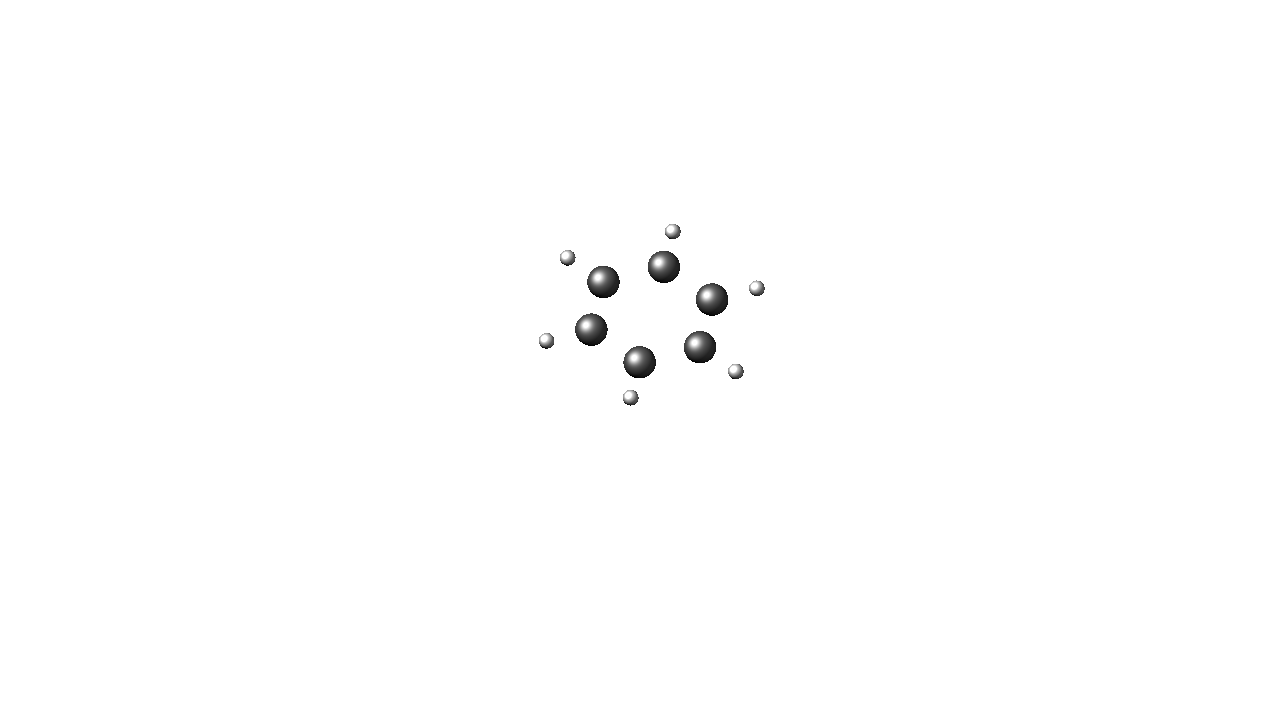
\includegraphics[width=0.40\textwidth]{c06h06}
	\bicaption{\enspace 这是一个样图}{\enspace This is a sample figure}
	\fignote{对图片的注释}

	\label{appfig:1}
	\stepcounter{app_fig}
\end{appfig}

% appendix content

\thispagestyle{appendixheader}
\backmatter% initialize the environment
%---------------------------------------------------------------------------%
%->> Backmatter
%---------------------------------------------------------------------------%
\chapter[致谢]{致\quad 谢}\chaptermark{致\quad 谢}% syntax: \chapter[目录]{标题}\chaptermark{页眉}
%\thispagestyle{noheaderstyle}% 如果需要移除当前页的页眉
%\pagestyle{noheaderstyle}% 如果需要移除整章的页眉

此处填写致谢。


\rightline{2023年6月}
\chapter{作者简历及攻读学位期间发表的学术论文与其他相关学术成果}

\section*{作者简历:}
××××年××月——××××年××月,在××大学××院(系)获得学士学位。

××××年××月——××××年××月,在××大学××院(系)获得硕士学位。

××××年××月——××××年××月,在中国科学院××研究所(或中国科学院大学××院系)攻读博士/硕士学位。

工作经历:

\section*{已发表(或正式接受)的学术论文:}

{
\setlist[enumerate]{}% restore default behavior
\begin{enumerate}[nosep]
    \item 已发表的工作1
    \item 已发表的工作2
\end{enumerate}
}

\section*{申请或已获得的专利:}

(无专利时此项不必列出)

\section*{参加的研究项目及获奖情况:}


\cleardoublepage[plain]% 让文档总是结束于偶数页,可根据需要设定页眉页脚样式,如 [noheaderstyle]
%---------------------------------------------------------------------------%
% other information
\end{document}
%---------------------------------------------------------------------------%

